\subsection{Experiment Two}\label{subsec:exp_two}

The second experiment investigated \cref{RQ:RQ2}, in order to identify our preferred measuring instrument on Windows. The measuring instrument was chosen based on a combination of different factors, including its correlation with our ground truth, ease of use and cost. 

A couple of changes were made in the experimental setup for experiment two. Firstly, due to some issues with SCAP, where its sampling rate significantly decreased when the DUT was under full load, the process priority class of the test case was set to \texttt{Normal}. Secondly, due to an execution time of less than a second for \texttt{MB} when compiled on Intel's oneApi, \texttt{MB's} input parameter was changed from $16.000$ to $64.000$ which increased the duration of the test case execution time to $\sim 14$ seconds. This avoided a scenario where the Plug only had a single data point per measurement. For this experiment, \texttt{FR} was executed $550$ times, while \texttt{MB} was executed $222$ times, based on \cref{tab:initial-measurements}.

\paragraph{Initial Measurements:} Following the initial measurements, Cochran's formula was applied as shown in \cref{app:exp_two_coch}. %In the cases where there were not enough measurements, the number from Cochran's formula was used to decide how many measurements each measuring instrument needed respectively. 
The Clamp required the most measurements, where the highest case required $44.106$ measurements. Since the number was significantly higher than the other test case and measuring instrument configurations, with the second highest being $4942$. An in depth look was taken into this configuration. In \cref{fig:evolution_of_medians} boxplots showing the evolution measurements can be seen when executing $100-1000$ measurements. The median decreased by $3.38\%$ from $100$ measurements to $1000$ measurements, and by $1.03\%$ between $900$ and $1000$ measurements. A pattern can be observed, where the median decreased as more measurements are made. Another pattern that can be observed is how the whisker increase in width as more measurement are taken. It can also be observed that the data is left skewed. However as more measurements are conducted the distribution evolves towards a more symmetric distribution. Due to the excessive time required to run the experiments, we have capped the maximum amount of measurement at $1000$.
%, but given how little the median changes, the argument is made that if Cochran's formula states that more than $1.000$ measurements are required, it will be capped at that.

\begin{figure}[H]
    \centering
    \begin{tikzpicture}[]
        \pgfplotsset{
            width=0.4\textwidth,
            height=0.30000000000000004\textheight
        }
        \begin{axis}[
            xlabel={Total Energy Consumption (Joules)}, 
            title={The evolution of energy consumption}, 
            ytick={1, 2, 3, 4, 5, 6, 7, 8, 9, 10},
        yticklabels={
            100, 200, 300, 400, 500, 600, 700, 800, 900, 1000
            },
            xmin=0,xmax=900,
            ]
        
        
        \addplot+ [boxplot prepared={
                lower whisker=590.5454367370409,
                lower quartile=678.0780564138329,
                median=725.6909322637096,
                upper quartile=736.564925883102,
                upper whisker=768.9024040272608
                }, color = red
                ] coordinates{(0,568.9963064028956)(0,577.3889614501314)(0,580.5219523454895)(0,558.138465719811)(0,566.0186537512344)(0,558.505322947511)(0,578.5466545316705)(0,575.2369758116332)(0,582.9138898275368)(0,586.4645553149074)(0,570.6944251769947)(0,573.1943482554922)(0,559.7777972478947)(0,562.44093838776)};
        
        \addplot+ [boxplot prepared={
                lower whisker=546.9587048609984,
                lower quartile=596.9198828215046,
                median=722.8583247095457,
                upper quartile=732.8970209692043,
                upper whisker=772.6368526958612
                }, color = red
                ] coordinates{};
        
        \addplot+ [boxplot prepared={
                lower whisker=546.3602044284822,
                lower quartile=596.7953970447156,
                median=720.9483710474394,
                upper quartile=735.9983653722971,
                upper whisker=795.2095113909105
                }, color = red
                ] coordinates{};
        
        \addplot+ [boxplot prepared={
                lower whisker=546.3602044284822,
                lower quartile=600.2181349376747,
                median=721.3156195144975,
                upper quartile=738.2456250999464,
                upper whisker=797.5048201967153
                }, color = red
                ] coordinates{};
        
        \addplot+ [boxplot prepared={
                lower whisker=546.3602044284822,
                lower quartile=609.8516239146488,
                median=721.0005528007746,
                upper quartile=741.4759980280355,
                upper whisker=797.5048201967153
                }, color = red
                ] coordinates{};
        
        \addplot+ [boxplot prepared={
                lower whisker=546.3602044284822,
                lower quartile=612.5915102527833,
                median=721.0005528007746,
                upper quartile=745.1087954064278,
                upper whisker=797.5048201967153
                }, color = red
                ] coordinates{};
        
        \addplot+ [boxplot prepared={
                lower whisker=546.3602044284822,
                lower quartile=612.4553381690396,
                median=720.8513174499045,
                upper quartile=746.148332399762,
                upper whisker=797.5048201967153
                }, color = red
                ] coordinates{};
        
        \addplot+ [boxplot prepared={
                lower whisker=546.3602044284822,
                lower quartile=611.5483474535424,
                median=713.3247210737799,
                upper quartile=745.352764089524,
                upper whisker=797.5048201967153
                }, color = red
                ] coordinates{};
        
        \addplot+ [boxplot prepared={
                lower whisker=474.33807947656385,
                lower quartile=610.0307582902374,
                median=708.7059666664006,
                upper quartile=745.4646354444801,
                upper whisker=827.6205569334105
                }, color = red
                ] coordinates{};
        
        \addplot+ [boxplot prepared={
                lower whisker=474.33807947656385,
                lower quartile=611.4375987908479,
                median=701.5053336410954,
                upper quartile=745.4646354444801,
                upper whisker=827.6205569334105
                }, color = red
                ] coordinates{};
        
        
        \end{axis}
    \end{tikzpicture}
\caption{A visual representation of how the energy measurements evolve as more measurements are made by clamp WIN on DUT 2 for test case MB} \label{fig:evolution_of_medians}
\end{figure}

\paragraph{Results:} When analyzing the results, graphs will be shown for the DEC for DUT 1, where additional plots can be found in \cref{app:exp_two}.

\begin{figure}[H]
    \centering
    \begin{tikzpicture}[]
        \pgfplotsset{
            width=0.9\textwidth,
            height=0.16\textheight
        }
        \begin{axis}[
            xlabel={DEC (Joules)}, 
            % title={The DEC of the CPU}, 
            ytick={1, 2, 3},
        yticklabels={
            4P, 2P2E, 4E
            },
            xmin=0,xmax=9000,
            ]
        
        
        \addplot+ [boxplot prepared={
                lower whisker=6647.178017561816,
                lower quartile=6683.891650872347,
                median=6823.3999122824625,
                upper quartile=7005.796515042039,
                upper whisker=7243.928965021686
                }, color = red
                ] coordinates{};
        
        \addplot+ [boxplot prepared={
                lower whisker=6522.216873120316,
                lower quartile=6657.345919263173,
                median=6873.2452374129825,
                upper quartile=7038.382427575665,
                upper whisker=7296.4127732030975
                }, color = red
                ] coordinates{};
        
        \addplot+ [boxplot prepared={
                lower whisker=7743.136290079687,
                lower quartile=7938.039832153479,
                median=8074.310191715255,
                upper quartile=8327.871004067803,
                upper whisker=8661.609332566171
                }, color = red
                ] coordinates{};
        
        
        \end{axis}
    \end{tikzpicture}
% \caption{CPU measurements by IPG on DUT 2 for test case(s) PCM compiled on } \label{fig:3-compare-p-and-e-cores-on-pcmark-with-boost-update-ipg-pc-mark-10.exe-unkown-workstationtwo-cpu-dec}
\end{figure}
\begin{figure}[H]
    \centering
    \begin{tikzpicture}[]
        \pgfplotsset{
            width=0.9\textwidth,
            height=0.16\textheight
        }
        \begin{axis}[
            xlabel={DEC (Joules)}, 
            % title={The DEC of the CPU}, 
            ytick={1, 2, 3},
        yticklabels={
            4P, 2P2E, 4E
            },
            xmin=0,xmax=9000,
            ]
        
        
        \addplot+ [boxplot prepared={
                lower whisker=6647.178017561816,
                lower quartile=6683.891650872347,
                median=6823.3999122824625,
                upper quartile=7005.796515042039,
                upper whisker=7243.928965021686
                }, color = red
                ] coordinates{};
        
        \addplot+ [boxplot prepared={
                lower whisker=6522.216873120316,
                lower quartile=6657.345919263173,
                median=6873.2452374129825,
                upper quartile=7038.382427575665,
                upper whisker=7296.4127732030975
                }, color = red
                ] coordinates{};
        
        \addplot+ [boxplot prepared={
                lower whisker=7743.136290079687,
                lower quartile=7938.039832153479,
                median=8074.310191715255,
                upper quartile=8327.871004067803,
                upper whisker=8661.609332566171
                }, color = red
                ] coordinates{};
        
        
        \end{axis}
    \end{tikzpicture}
% \caption{CPU measurements by IPG on DUT 2 for test case(s) PCM compiled on } \label{fig:3-compare-p-and-e-cores-on-pcmark-with-boost-update-ipg-pc-mark-10.exe-unkown-workstationtwo-cpu-dec}
\end{figure}

When applying statistical methods from \cref{subsec:Statistics}, it was discovered that some of the data did not follow a normal distribution and were significantly different from eachother, previous studies \cite{biksbois, Koedijk2022diff} have had simliar results. Thus, Kendalls Tau Correlation Coefficient was used, and the results for the two test cases can be seen in \cref{fig:fannkuchCorr} and \cref{fig:mandelbrotCorr}.

\begin{figure}[H]
    \centering
    \hspace*{-1cm} % move the figure 1cm to the left
    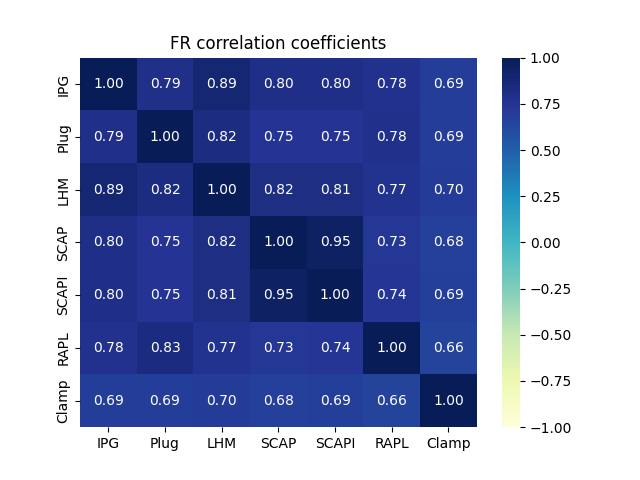
\includegraphics[width=0.6\textwidth]{figures/Fannkuch-redux_ex2.png}
    \caption{Heatmap showing the correlation ceoffecient betwween all of the measurement instrument on windows for the fannkuch-redux testcase}
    \label{fig:fannkuchCorr}
  \end{figure}
  
  \begin{figure}[H]
    \centering
    \hspace*{-1cm} % move the figure 1cm to the left
    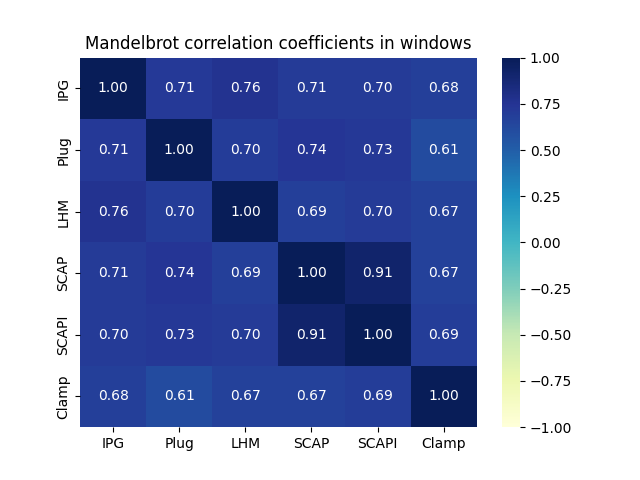
\includegraphics[width=0.6\textwidth]{figures/Mandelbrot_ex2.png}
    \caption{Heatmap showing the correlation coefficient between all of the measurement instruments on windows for the Mandelbrot test case.}
    \label{fig:mandelbrotCorr}
  \end{figure}
  

  All DUTs showed moderate to high correlation with the ground truth (Clamp) when assessed with the Guildford Scale. The measuring instruments varied in their correlation performance, with SCAPI being the best but with very few data points logged, this is also the case with SCAP. LHM and IPG being essentially equal in performance for both test cases which Slight diviations. Since usability is also a factor, IPG was chosen as the best measuring instrument and will be used for future experiments on Windows.


